% Opening: two routes to the same submitted proof. The student's own work and
% an exchange with a chatbot sit inside a dashed box; only the page leaves it.
\documentclass[tikz,border=6pt]{standalone}
% Shared art for "Asking a chatbot to confirm a proof": the palette and the
% chatbot, worksheet and chat bubble of the SPLICE talk's summary figure and
% the Builder tile, so the post, the talk page and the lab page look alike.
\usetikzlibrary{arrows.meta,decorations.pathmorphing,calc}
\definecolor{ink}{HTML}{1B2430}
\definecolor{rule}{HTML}{9AA4AB}
\definecolor{edge}{HTML}{5A646E}
\definecolor{tint}{HTML}{F7E9E9}
\definecolor{red}{HTML}{8B2E2E}
\tikzset{
  flow/.style={-{Stealth[length=3.4mm]}, draw=edge, line width=1.3pt},
  lbl/.style={font=\sffamily\Large, text=ink, align=center},
  note/.style={font=\sffamily\large, text=edge, align=center},
  title/.style={font=\sffamily\bfseries\LARGE, text=ink},
  chip/.style={font=\sffamily\bfseries\large, text=white, fill=red,
               rounded corners=3pt, inner sep=5pt},
}
% A worksheet: lower-left (#1,#2), width #3, height #4. #5 is the colour of the
% third line: red for a perturbed question, rule for plain work.
\newcommand{\sheet}[5]{%
  \fill[white, draw=edge, line width=1.2pt, line join=round]
    (#1,#2) -- ++(#3,0) -- ++(0,#4-0.4) -- ++(-0.4,0.4) -- ++(-#3+0.4,0) -- cycle;
  \draw[edge, line width=1.2pt, line join=round] (#1+#3-0.4,#2+#4) -- ++(0,-0.4) -- ++(0.4,0);
  \foreach \f in {0.76,0.58,0.24}
    \draw[rule, line width=1.5pt, line cap=round] (#1+0.28,#2+\f*#4) -- ++(#3-0.56,0);
  \draw[#5, line width=1.7pt, line cap=round, decorate,
        decoration={zigzag, segment length=2.2mm, amplitude=0.7mm}]
    (#1+0.28,#2+0.41*#4) -- ++(#3-0.56,0);}
% The chatbot's head, centred on (#1,#2).
\newcommand{\chatbot}[2]{%
  \fill[red] (#1-0.8,#2-0.62) rectangle ++(1.6,1.24);
  \fill[white] (#1-0.4,#2+0.12) circle (0.16);
  \fill[white] (#1+0.4,#2+0.12) circle (0.16);
  \draw[white, line width=1.3pt] (#1-0.3,#2-0.3) -- ++(0.6,0);
  \draw[red, line width=1.5pt] (#1,#2+0.62) -- ++(0,0.4);
  \fill[red] (#1,#2+1.1) circle (0.13);}
% A student: head and shoulders, centred on (#1,#2).
\newcommand{\student}[2]{%
  \fill[edge] (#1,#2+0.45) circle (0.42);
  \fill[edge] (#1-0.8,#2-0.75) .. controls (#1-0.8,#2+0.1) and (#1+0.8,#2+0.1) .. (#1+0.8,#2-0.75) -- cycle;}
% A rubric card, failed, lower-left (#1,#2), side #3.
\newcommand{\failcard}[3]{%
  \fill[white, draw=edge, line width=1.2pt, rounded corners=3pt] (#1,#2) rectangle ++(#3,#3);
  \draw[red, line width=2.6pt, line cap=round]
    (#1+0.25*#3,#2+0.25*#3) -- ++(0.5*#3,0.5*#3) (#1+0.25*#3,#2+0.75*#3) -- ++(0.5*#3,-0.5*#3);}

\begin{document}
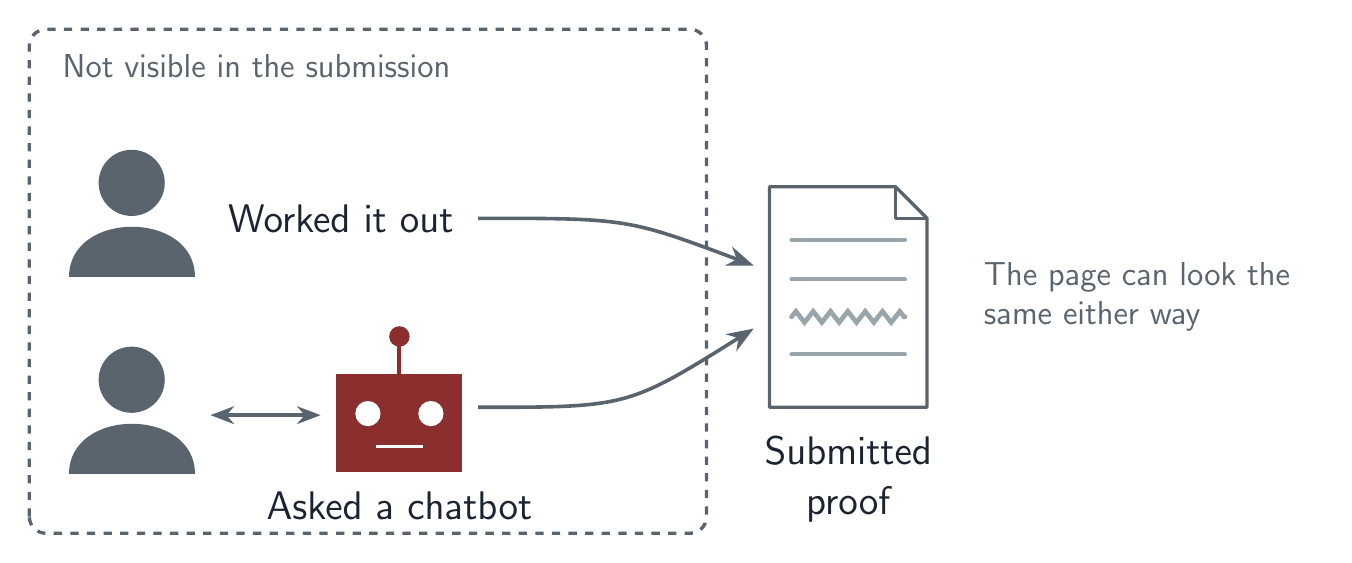
\begin{tikzpicture}[font=\sffamily]
  \draw[edge, line width=1.2pt, dashed, rounded corners=6pt] (0,0) rectangle (8.6,6.4);
  \node[note, anchor=north west] at (0.3,6.2) {Not visible in the submission};
  % route 1: the student works it out
  \student{1.3}{4.0}
  \node[lbl, anchor=west] at (2.4,4.0) {Worked it out};
  % route 2: the student asks a chatbot
  \student{1.3}{1.5}
  \draw[edge, line width=1.3pt, {Stealth[length=3mm]}-{Stealth[length=3mm]}] (2.3,1.5) -- (3.7,1.5);
  \chatbot{4.7}{1.4}
  \node[lbl, anchor=north] at (4.7,0.65) {Asked a chatbot};
  \draw[flow] (5.7,4.0) .. controls (7.6,4.0) .. (9.2,3.4);
  \draw[flow] (5.7,1.6) .. controls (7.6,1.6) .. (9.2,2.6);
  % the one thing that leaves the box
  \sheet{9.4}{1.6}{2.0}{2.8}{rule}
  \node[lbl, anchor=north] at (10.4,1.35) {Submitted\\proof};
  \node[note, anchor=west, text width=4.2cm, align=left] at (12.0,3.0) {The page can look the same either way};
\end{tikzpicture}
\end{document}
